\begin{savequote}[75mm]
   If I model a phenomenon accurately, does that mean I understand it? Or might it be simple coincidence, or an artifact
   of the technique? Of course, as an ardent simulationist, I myself put much faith in Engine-modeling.
\qauthor{Edward Mallory, The Difference Engine by William Gibson and Bruce Sterling}
\end{savequote}

\chapter{Wyniki}

\subsection{Liniowa analiza stabilności}
\label{sec:lsa}
Jednym z celów naukowych poniższej pracy jest walidacja wyników eksperymentu
numerycznego poprzez porównanie z tempem wzrostu najsilniejszych modów
otrzymanych z liniowej analizy stabilności. W tym rozdziale przedstawiono
poszczególne kroki liniowej analizy stabilności dla niestabilności strumieniowej
w oparciu o pracę~\citep{YG05}.

Analiza stabilności opiera się na trzech elementach:
\begin{enumerate}
   \item znalezieniu stanu równowagi dla zadanego układu równań,
   \item zaburzeniu układu znaną funkcją o małej amplitudzie 
   \item wyprowadzeniu modów własnych oraz ich tempa wzrostu.
\end{enumerate}
Niestety dla układu równań hydrodynamiki dwóch sprzężonych płynów w rozciągłym
dysku keplerowskim nie istnieje warunek równowagowy. Spowodowane jest to
migracja pyłu na centrum grawitacji na skutek utraty momemtu pędu przez tarcie
aerodynamiczne. Naturalną konsekwencją migracji są znaczne zmiany w radialnym
profilu rozkładu gęstości pyłu. Należy jednak zauważyć, że charakterystyczna
skala czasowa migracji jest rzędu setek bądź wiecej lat, przy założeniu iż mamy
do czynienia z aglomeratami pyłu o rozmiarach metrowych. Z tego względu możemy
założyć że zmiany w profilu gęstości są procesem powolnym w stosunku do typowego
tempa wzrostu niestabilności strumieniowej, co zostanie wykazane w dalszej
części wywodu.

Kolejną przeszkodą jest sama rozciągłość symulowanego dysku okołogwiazdowego,
która implikuje zmienność potencjalnego stanu równowagowego wraz z promieniem
dysku. W tym wypadku powinno przeprowadzić się globalną analizę stabilności po
przez rozwiązanie dwupunktowego problem brzegowego (np.~\cite{PHM04, KH06}),
jednakże takie podejście jest dużo bardziej skomplikowane. Przedstawianą tu
lokalną analizę należy zatem traktować jako pierwsze przybliżenie pełnej analizy
stabilności niestabiności strumieniowej. Niestabilne mody uzyskane w ramach
liniowej analizy posłużą nam jako punkt odniesienia dla modów uzyskiwanych w
globalnym eksperymencie numerycznym.

Najbardziej wygodnym układem do lokalnego opisu niestabilności strumieniowej
jest tzw. kostka ścinana~\footnote{ang. shearing box}~\citep{HGB95}, czyli
kartezjański układ współrzędnych, którego początek współporusza się z płynem na
wybranej orbicie $R_0$ z częstością keplerowską $\Omega_0 \equiv
\Omega\left(R_0\right)$. Zwyczajowo przyjmuje się, że oś $x$ jest skierowana
radialnie na zewnątrz, oś $y$ jest w kierunku azymutalnym, zaś $z$ jest osią
wertykalną. Zgodnie z pracą~\cite*{YJ07} układ równań ciągłości oraz ruchu dla
obu składników można wyrazić poprzez:
%
\begin{align}
\partial_t \rho_g &+ \mathbf{u}\cdot\nabla\rho_g - \frac{3}{2}\Omega x\partial_y\rho_g 
 = -\rho_g\nabla\cdot\mathbf{u},\label{eqc1}\\
\partial_t \rho_d &+ \mathbf{w}\cdot\nabla\rho_d - \frac{3}{2}\Omega x\partial_y\rho_d 
 = -\rho_d\nabla\cdot\mathbf{w},\label{eqc2}\\
\partial_t \mathbf{u} &+ \left(\mathbf{u}\cdot\nabla\right)\mathbf{u} 
 - \frac{3}{2}\Omega x\partial_y\mathbf{u} 
 = 2\Omega u_y \hat{\mathbf{x}} -\frac{1}{2}\Omega u_x \hat{\mathbf{y}} \notag\\
 &- \frac{\epsilon}{\tau_f}(\mathbf{u}-\mathbf{w}) -c_s^2\nabla\ln\rho_g 
 +2\eta\Omega^2 R \hat{\mathbf{x}},\label{eqm1}\\
\partial_t \mathbf{w} &+ \left(\mathbf{w}\cdot\nabla\right)\mathbf{w} 
 - \frac{3}{2}\Omega x\partial_y\mathbf{w}
 = 2\Omega w_y \hat{\mathbf{x}} -\frac{1}{2}\Omega w_x \hat{\mathbf{y}} \notag\\
 &- \frac{1}{\tau_f}(\mathbf{w}-\mathbf{u}), \label{eqm2}
\end{align}
%
gdzie wyrazy takie jak $(3/2)\Omega x$ po lewej stronie równań, pojawiają się na
skutek relatywizacji wszytkich predkości względem liniowego, ścinanego przepływu
$\mathbf{v}_0 = -(3/2)\Omega x \hat{\mathbf{y}}$ w rotującym układzie
współrzędnych. Warto nadmienić, że wyraz $-(1/2)\Omega \{u,w\}_x
\hat{\mathbf{y}}$ po prawej stronie równań ruchu \mref{eqm1}-\mref{eqm2} jest
sumą dwóch składników: $(-2\Omega \{u,w\}_x + (3/2)\Omega \{u,w\}_x)
\hat{\mathbf{y}}$ z których pierwszy jest składową siły Coriolisa, a drugi
wynika z odjęcia wspomnianego wcześniej przepływu średniego. Główną różnicą
pomiędzy równaniami \mref{eqm1} oraz \mref{eqm2} jest brak wyrazu ciśnieniowego
dla składnika pyłowego. Jak zauważyli YG05, można w spójny sposób uwzględnić
globalny, radialny gradient ciśnienia gazu ograniczając się do liniowego wyrazu,
który jest zparametryzowany tzw. bezwymiarową miarą rotacji podkeplerowskiej:

\begin{equation}
\eta \equiv - \frac{\partial_R P}{2\rho_g\Omega^2 R} \sim \frac{c_s^2}{v_K^2}.
\end{equation}

Układ równań \mref{eqc1}-\mref{eqm2} posiada znane rozwiązanie równowagowe~\citep{N86}

\begin{align}
\bar{\mathbf{w}} &= \left[ 
 -2\tau_s\xi, \frac{\tau_s^2\xi - 1}{1+\epsilon},
 0
\right]\eta v_K, \label{eq:w0}\\
\bar{\mathbf{u}} &= \left[ 
 2\epsilon\tau_s\xi, -\frac{1 + \epsilon\tau_s^2\xi}{1+\epsilon},
 0
\right]\eta v_K, \label{eq:u0}
\end{align}
%
gdzie $\tau_s = \Omega \tau_f$ to dimensionless stopping time i 
$\xi = ((1+\epsilon)^2 + \tau_s^2)^{-1}$. 
Linearyzacja równań \mref{eqc1}-\mref{eqm2}, polega na rozbiciu zmiennych na
część stałą oraz zaburzenie $\mathbf{q} = \bar{\mathbf{q}} + \mathbf{q}^\prime$,
gdzie $\mathbf{q}=[\rho_d, w_x, w_y, w_z, \rho_g, u_x, u_y, u_z]$. Zakładamy
równocześnie, że zaburzenie jest osiowosymetryczne (niezależne od współrzędnej $y$)
i przyjmuje postać fali płaskiej:

\begin{equation}
   \label{eq:planar}
   \mathbf{q}^\prime(x,z,t) = \tilde{\mathbf{q}}
 \exp\left[i(k_x x + k_z z -\omega t)\right]
\end{equation}

Po podstawieniu liniowego zaburzenia układ równań przyjmuje następującą postać

\begin{align}
-i(\omega- k_x\bar{w}_x)\tilde{\rho}_d &= 
 - i \bar{\rho}_d(k_x\tilde{w}_x + k_z\tilde{w}_z), \label{lin1}\\
-i(\omega- k_x\bar{u}_x)\tilde{\rho}_g &= 
 - i \bar{\rho}_g(k_x\tilde{u}_x + k_z\tilde{u}_z), \label{lin2}\\
-i(\omega- k_x\bar{u}_x)\tilde{\mathbf{u}} &= 
 2\Omega \tilde{u}_y\hat{\mathbf{x}} - \frac{1}{2}\Omega \tilde{u}_x
 \hat{\mathbf{y}}
 -\frac{\epsilon}{\tau_f}(\tilde{\mathbf{u}} - \tilde{\mathbf{w}}) \notag\\
  -\frac{\tilde{\rho}_d}{\bar{\rho}_g\tau_f}
  (\bar{\mathbf{u}} &- \bar{\mathbf{w}})
  - \frac{c_s^2}{\bar{\rho}_g}ik_x\tilde{\rho}_g\hat{\mathbf{x}} -
  - \frac{c_s^2}{\bar{\rho}_g}ik_z\tilde{\rho}_g\hat{\mathbf{z}}, \label{lin3}\\
-i(\omega- k_x\bar{w}_x)\tilde{\mathbf{w}} &= 
 2\Omega \tilde{w}_y\hat{\mathbf{x}} - \frac{1}{2}\Omega \tilde{w}_x
 \hat{\mathbf{y}} 
 - \frac{1}{\tau_f} (\tilde{\mathbf{w}} - \tilde{\mathbf{u}}), \label{lin4}
\end{align}
%
gdzie $\epsilon = \bar{\rho}_d/\bar{\rho}_g$. Układ równań
\mref{lin1}-\mref{lin4} można zapisać jako

\begin{equation}
 \eurom{A}(k_x,k_z,\omega)\tilde{\mathbf{q}} = 0
 \label{eq:linset}
\end{equation}
%
Nietrywialne rozwiązania układu linoweg \mref{eq:linset} istnieją wtedy i tylko
wtedy gdy równanie dyspersyjne 
\begin{equation}
 \det|\eurom{A}(k_x,k_z,\omega)|=0.
 \label{eq:disprel}
\end{equation}
%
Dla zadanych wartości $(k_x, k_x)$ relację \mref{eq:disprel} można rozwiąć ze
względu na $\omega$ i dzięki temu otrzymać związki pomiędzy amplitudami
składowych wektora $\tilde{\mathbf{q}}$.
We solve the dispersion relation \mref{eq:disprel} for given values of
$(k_x,k_z)$, with respect to the complex frequency $\omega$, using the
Tempo wzrostu niestabilności definiujemy jako urojoną część zespolonej
częstotliwości $s=\Im(\omega)$.
%
\begin{figure*}
   \centering
   \begin{tabular}{@{}cc@{}}
      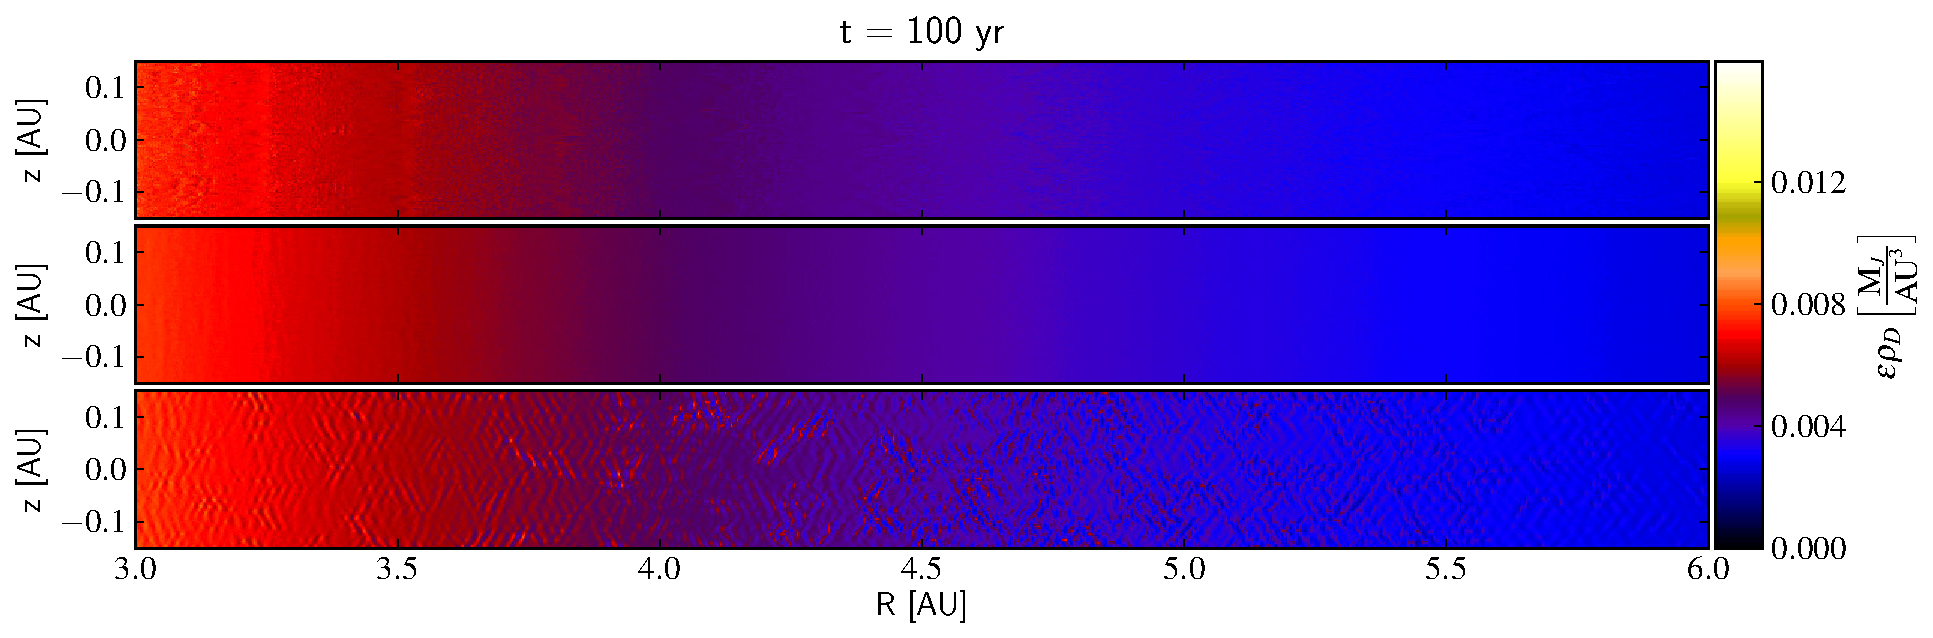
\includegraphics[width=0.49\linewidth]{figures/fig2a} &
      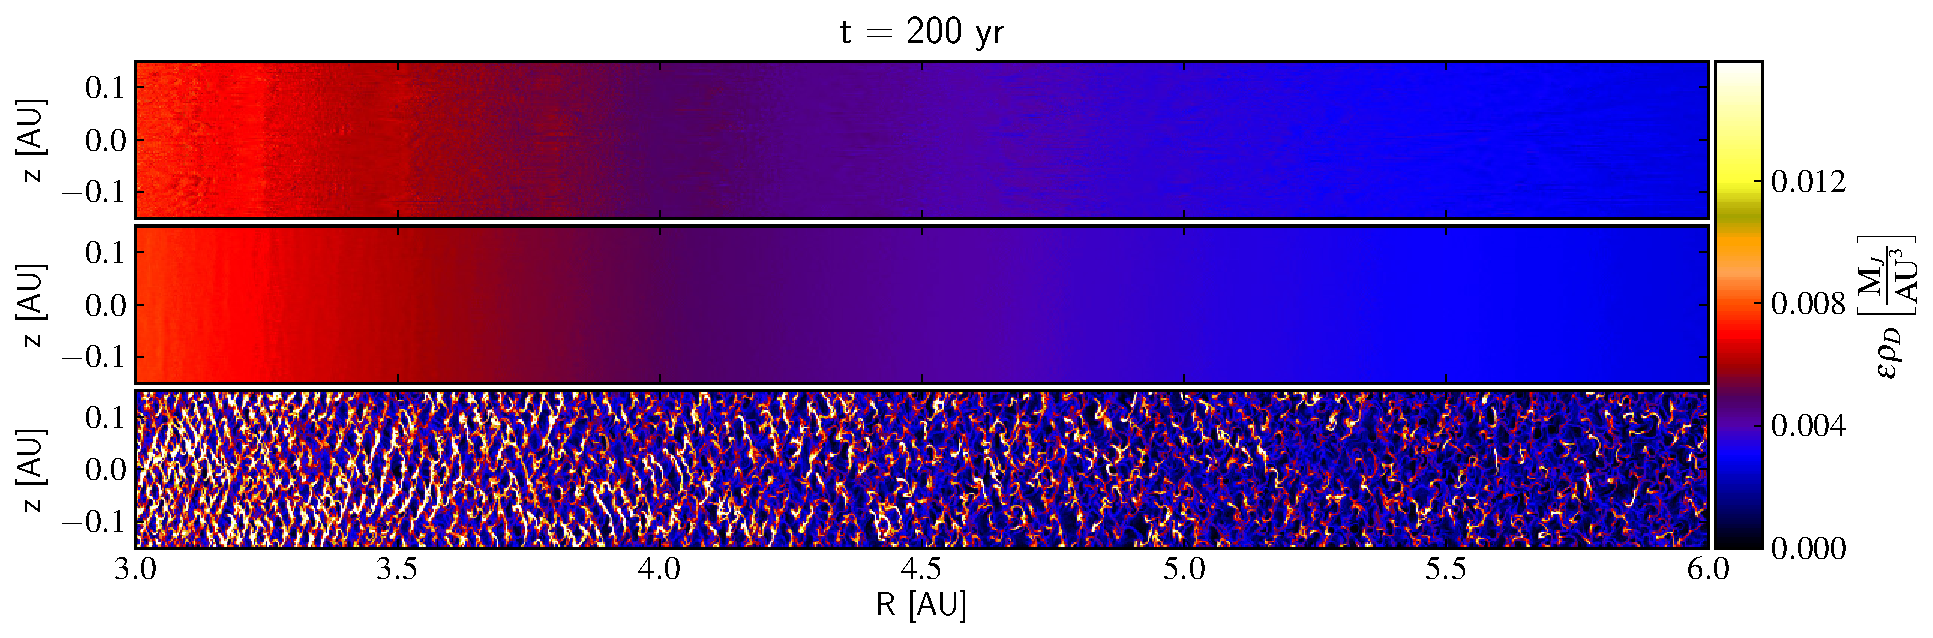
\includegraphics[width=0.49\linewidth]{figures/fig2b} \\
      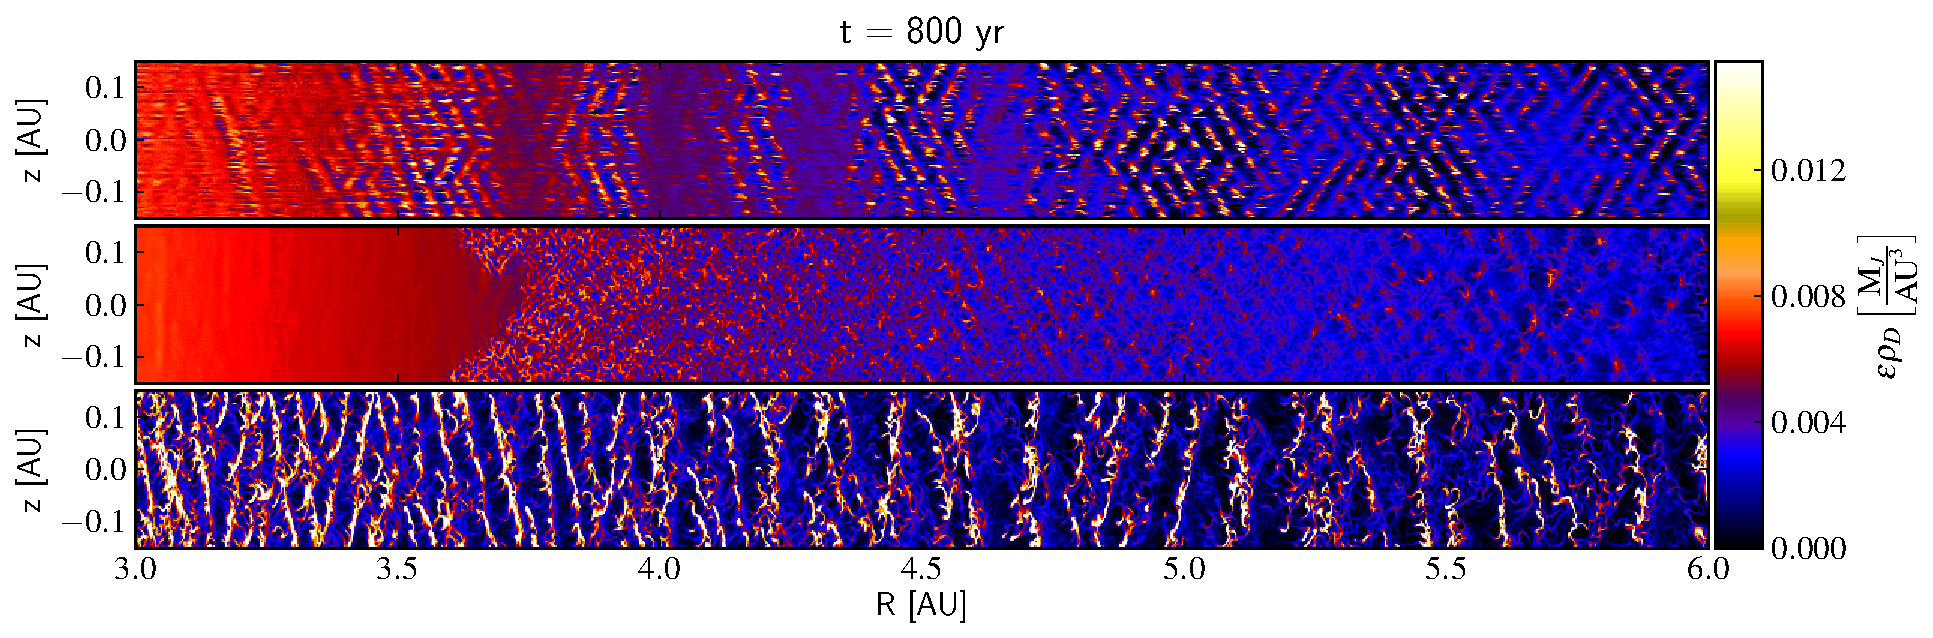
\includegraphics[width=0.49\linewidth]{figures/fig2c} &
      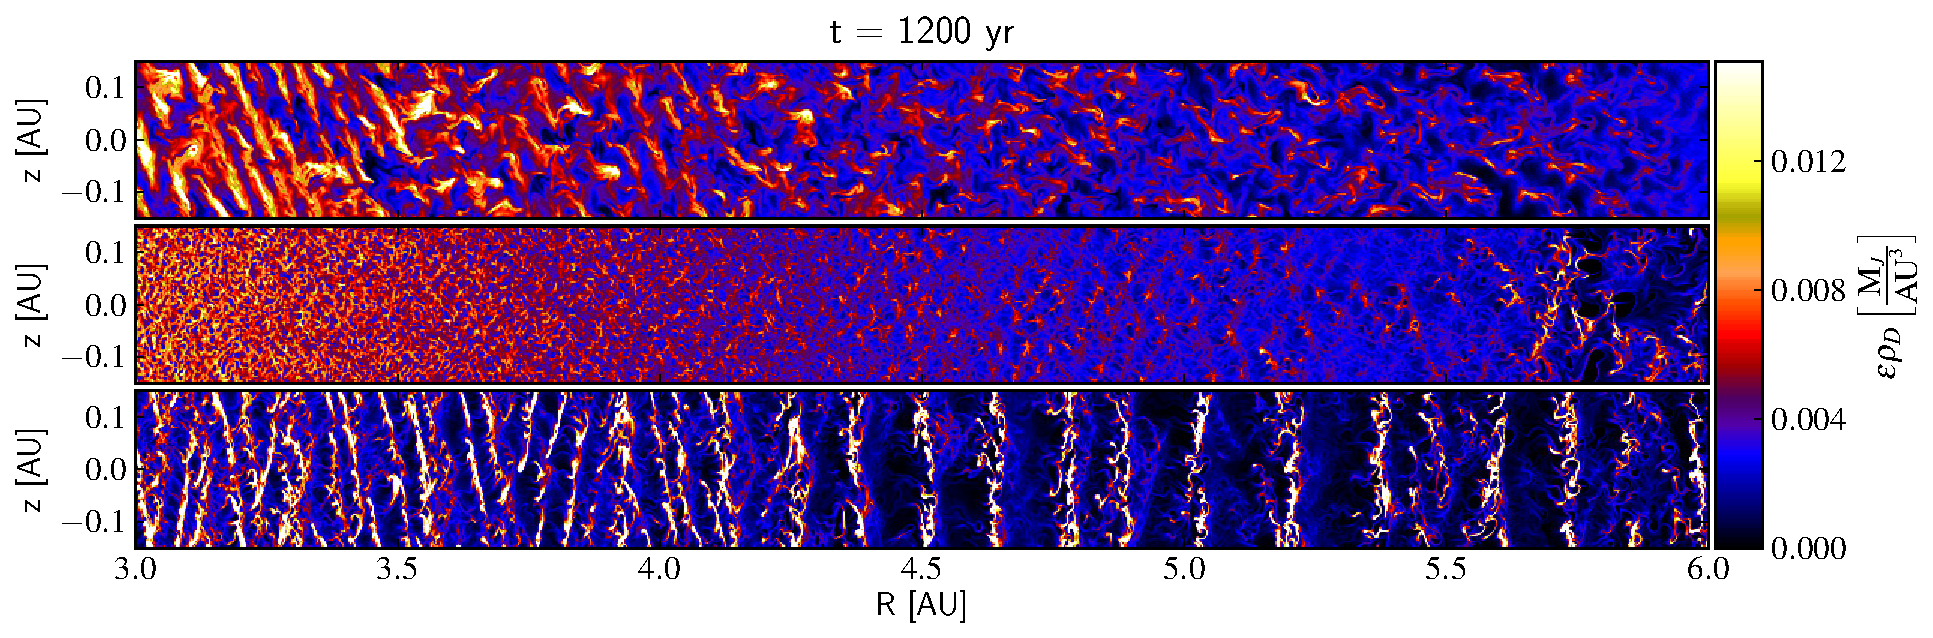
\includegraphics[width=0.49\linewidth]{figures/fig2d}
   \end{tabular}
   \caption{Migawki gęstości pyłu dla symulacji z $10$~cm ziarnami pyłu
      dla czasu $100$, $200$, $800$ oraz $1200$~lat odpowiednio dla lewego
      górnego, prawego górnego, dolnego lewego i dolnego prawego panelu.
      Każdy z paneli jest podzielony na trzy części różniące się początkowym 
      $\epsilon = 0.2, 1, 2.0$ odpowiednio dla górnego (AA), środkowego (AB) i
      dolnego (AC) podpanelu.}
   \label{fig2}
\end{figure*}

\label{sec:results}
The initial stage of streaming instability evolution is similar for all cases of
$\epsilon$ or $a$ and is governed by the dominant linear modes. Detailed
analysis of linear phase is covered in Section~\ref{simulation_analysis}. The
following two sections describe different non-linear evolution of streaming
instability in quasi-global setup with reference to similar case shown by JY07.
%
\subsection{Marginally Coupled Boulders}% ($a=50\,\textrm{cm}$, $\tau_s\approx
%1.2$)\label{marg_boulders}}
%
As noted by JY07, streaming instability is the most prominent for $\tau_s = 1$
and exhibits fast linear growth and heavy dust clumping.  Figure~\ref{fig1}
shows temporal evolution of streaming instability for different initial dust to
gas ratios $\epsilon$. In all cases (BA, BB, BC) elongated clumps are formed.
When the saturated state is reached, due to the high vertical speed of dust
overdensities, the filaments undergo occasional fragmentation and collisions
with each other, though still following "v"-shaped trajectories that emerged
during linear phase. The most prominent differences between BA, BB and BC are:
(1) the characteristic length of local clumps is decreasing with the increase of
initial $\epsilon$ and (2) their tendency to lean in radial direction: in BB
structures are almost purely diagonal, whereas in BA and BC are much more
elongated in the vertical direction.
Similarly to JY07, in all cases (BA, BB, BC) the density peaks of the dust
component in the non-linear regime settle at levels about 2 order of magnitude
higher than initial density.

\subsection{Tightly Coupled Boulders}
%($a=10\,\textrm{cm}$, $\tau_s\approx 0.24$)
%\label{tight_boulders}}

Since the fluid approach, contrary to the particle description, is much less
susceptible to effects of Poisson noise we were able to follow linear phase for
run AB and ABh for much longer than JY07, though in the end we also observe
sudden increase in growth rate of the instability due to spontaneous cavitation
(initial phase is caught in the middle subpanel of bottom right panel of
Fig.~\ref{fig2}).
The bubbles of void start to spawn at outer radii and greatly increase the dust
density and velocity on their edges (see Fig.~\ref{fig3}). After just
few orbital periods the accelerated instability expands to whole domain and
dominate the nonlinear evolution. Afterwards the quasi-stationary state of
vivid turbulence is achieved. 
In both cases (AB, AC), the non-linear evolution leads to the enhancement
of the peak densities of dust component over one order of magnitude, which is in
close agreement with results of JY07 (see Fig.~8 in their work).

\begin{figure} 
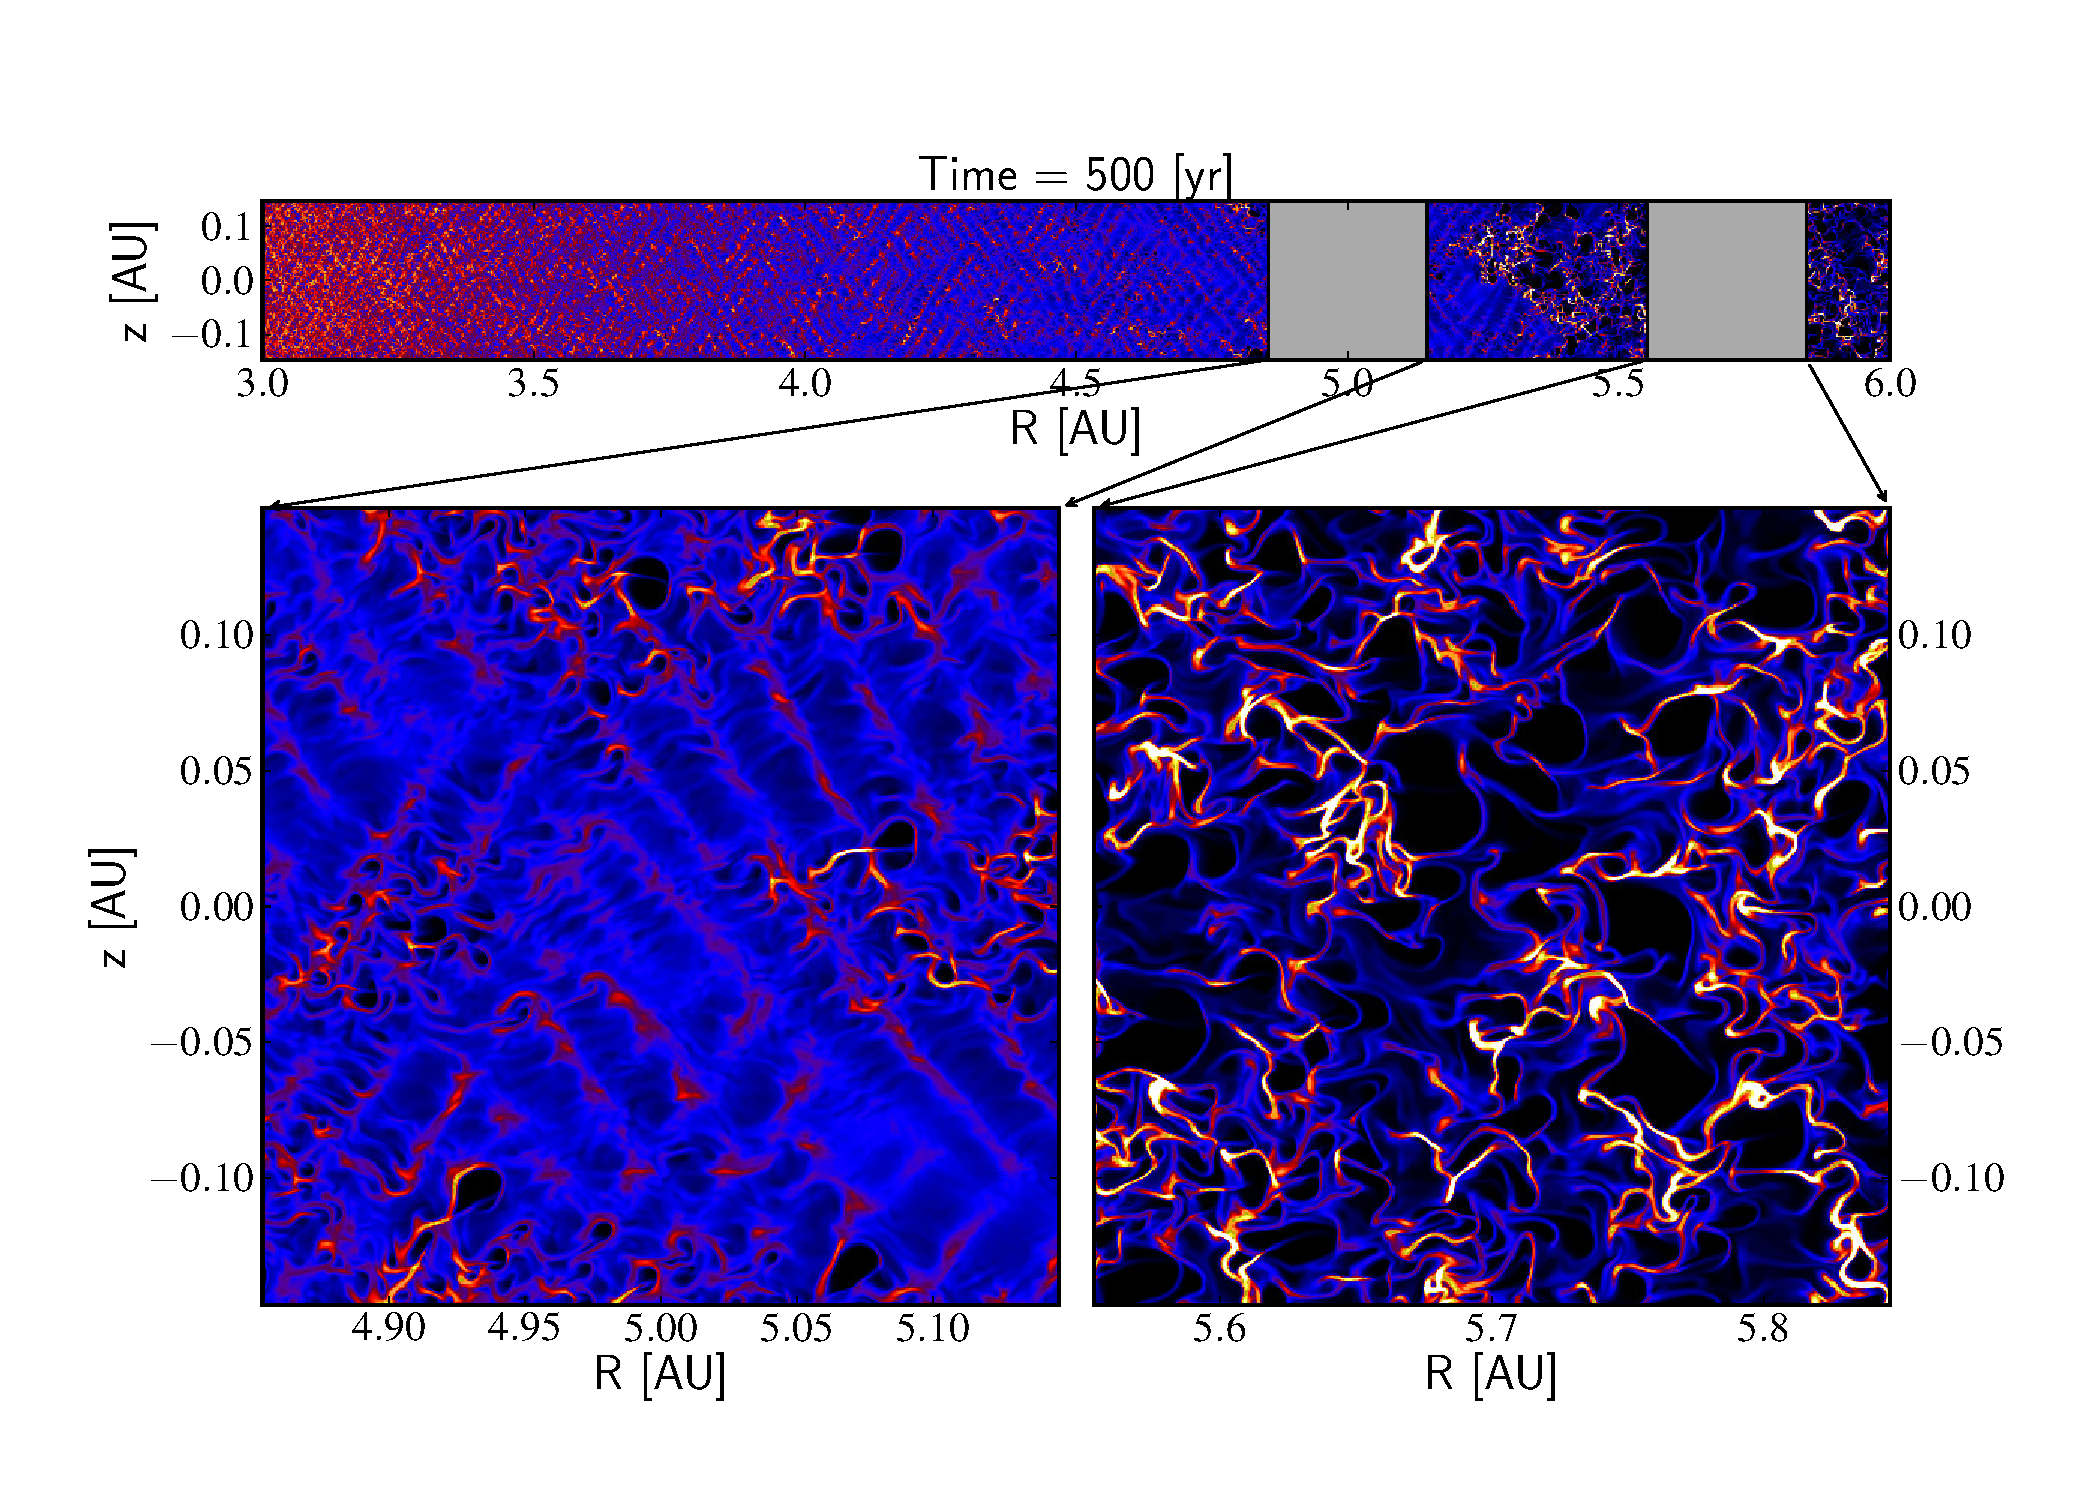
\includegraphics[width=0.98\linewidth]{figures/fig3}
\caption{Dust density snapshot for run ABh showing two "zoom-in" regions where
cavities emerge from overdensities created during linear phase of evolution
(left panel) and region totally overwhelmed by bursting void bubbles and vivid
dust turbulence (right panel). Animation of the run ABh can be found 
\href{http://youtu.be/NoA5-TiQabQ}{here}.}
\label{fig3}
\end{figure}

\par In the dust dominated case (AC) our results closely follow those of JY07 up
to the point of saturation, where we achieve highly turbulent flow (lower
subpanel of upper right panel of Fig.~\ref{fig2}) and about 20 fold growth
in dust density. However, we note that secular evolution of the physical system
leads to formation of elongated dust overdensities and further growth up to 2
orders of magnitude as seen in runs with other parameters (see lower subpanel of
bottom right panel of Fig.~\ref{fig2}).

\par In the gas dominated case (AA) we observe initial overdensity growth over
two orders of magnitude in a characteristic grid-like pattern.  However, at time
1200, 440, 325 for runs AA, AAh, AAu respectively, in the course of nonlinear
evolution the dense dust filaments are abruptly smoothed out resulting in
oscillatory motion of mild overdensities that are only one order of magnitude
denser than initial dust distribution (see Fig.~\ref{fig4})

\begin{figure}
   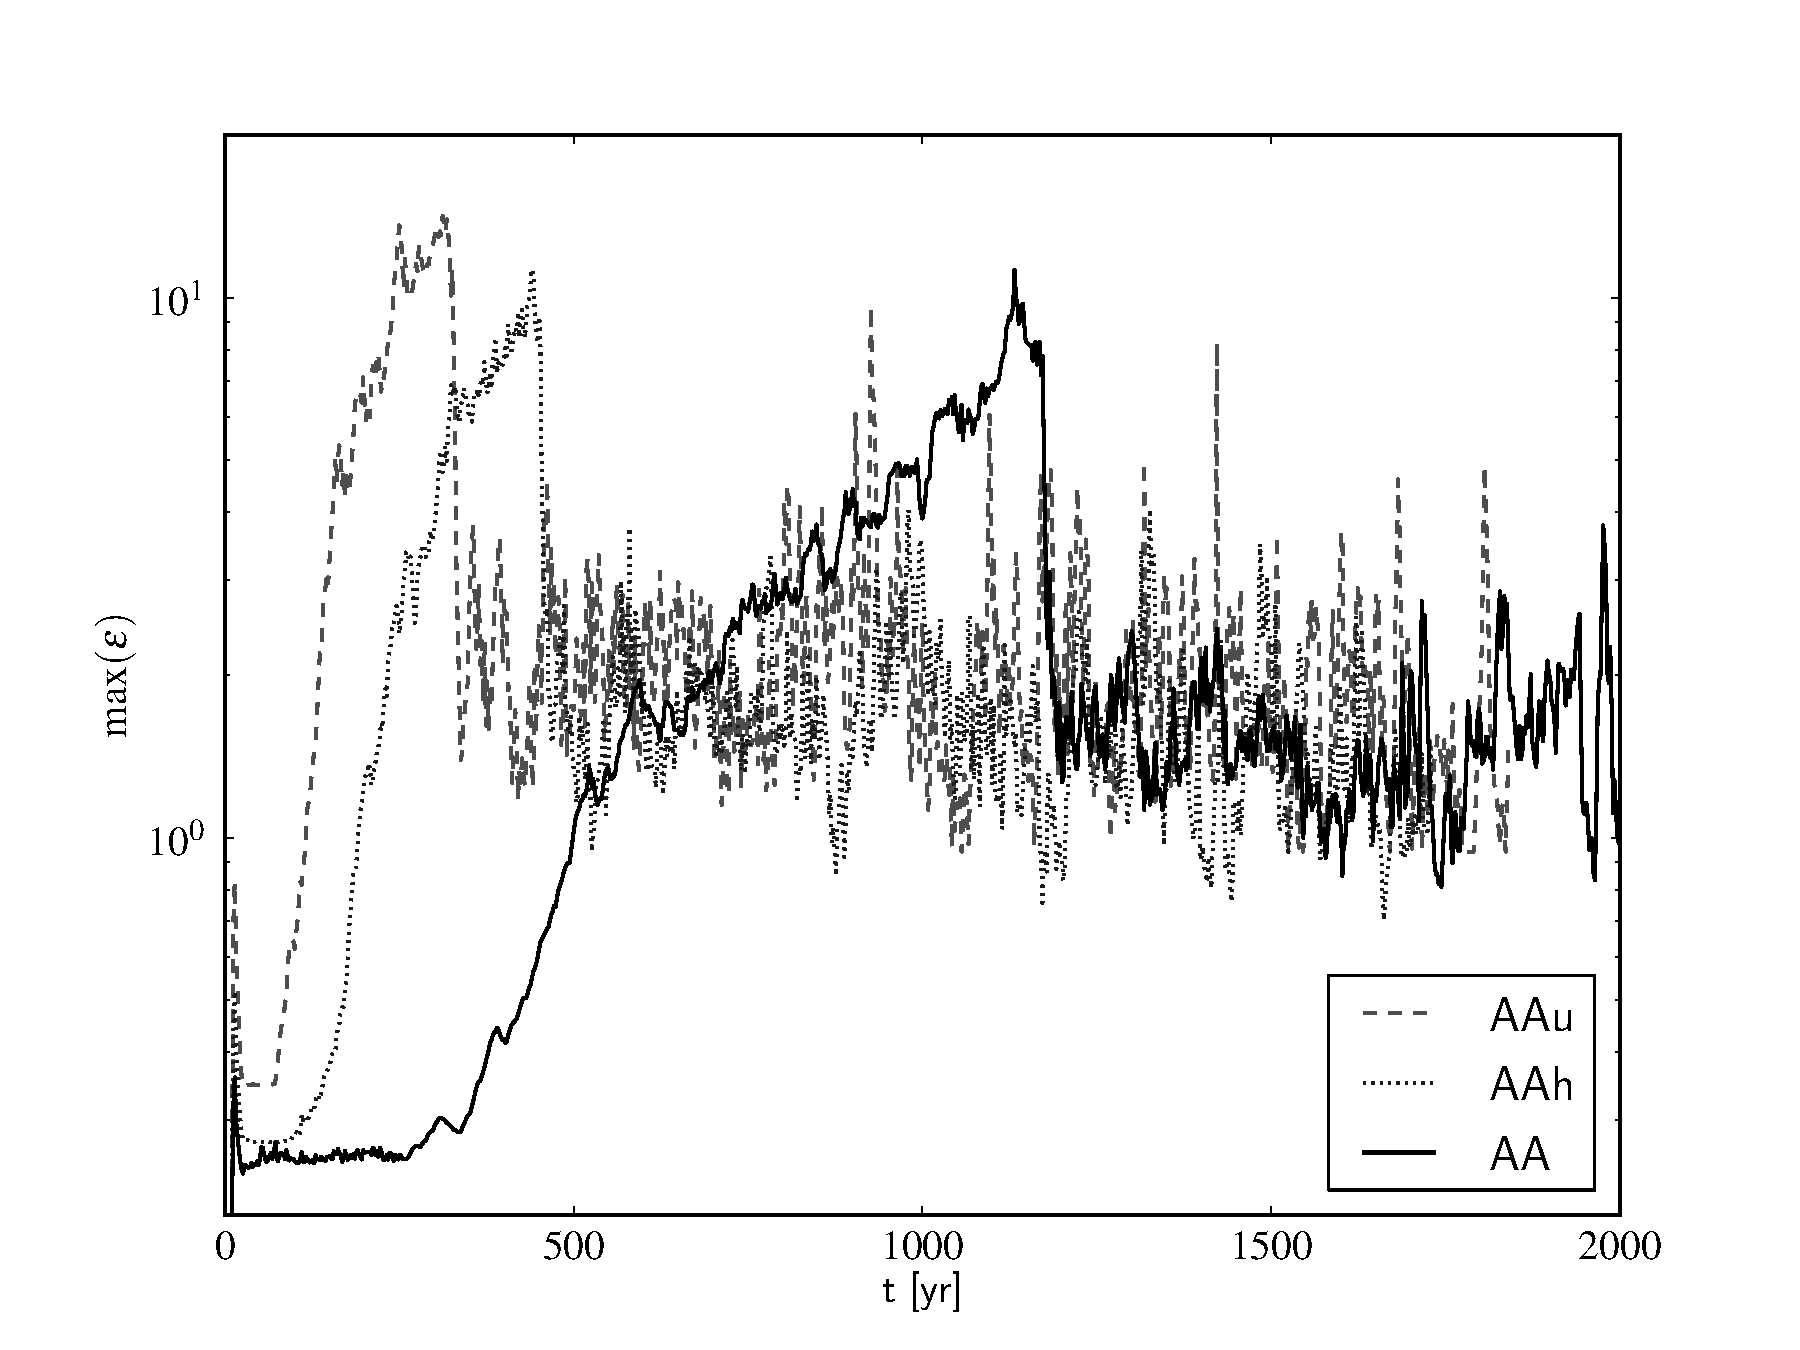
\includegraphics[width=0.98\linewidth]{figures/fig4}
   \caption{Maximum ratio of dust to gas density for three runs with the same
      initial conditions, but different resolution. Streaming instability
      follows regular pattern of evolution: (1) fast linear growth that locally
      increases $\epsilon$ over 2 orders of magnitude (2) after reaching certain
      level of $\epsilon \approx 10$, overdensities are abruptly smoothed out
      (3) instability reaches out saturated, non-linear phase where large,
      smooth clumps of dust are only 10 times denser than initial condition.
      Varying resolution only influences the availability of shorter and faster
      growing modes, i.e. shortens phase (1).  }
   \label{fig4}
\end{figure}
%
\subsection{3D run}
The course of the evolution of our single 3D (BB3D) closely follows the
corresponding 2D run BB (compare Fig.~\ref{fig5} and Fig.~\ref{fig1}). During
the linear phase of growth elongated clumps or rather sheets of dense dust are
formed, as the deviation from axis axisymmetry is almost negligible.
%
\begin{figure}
   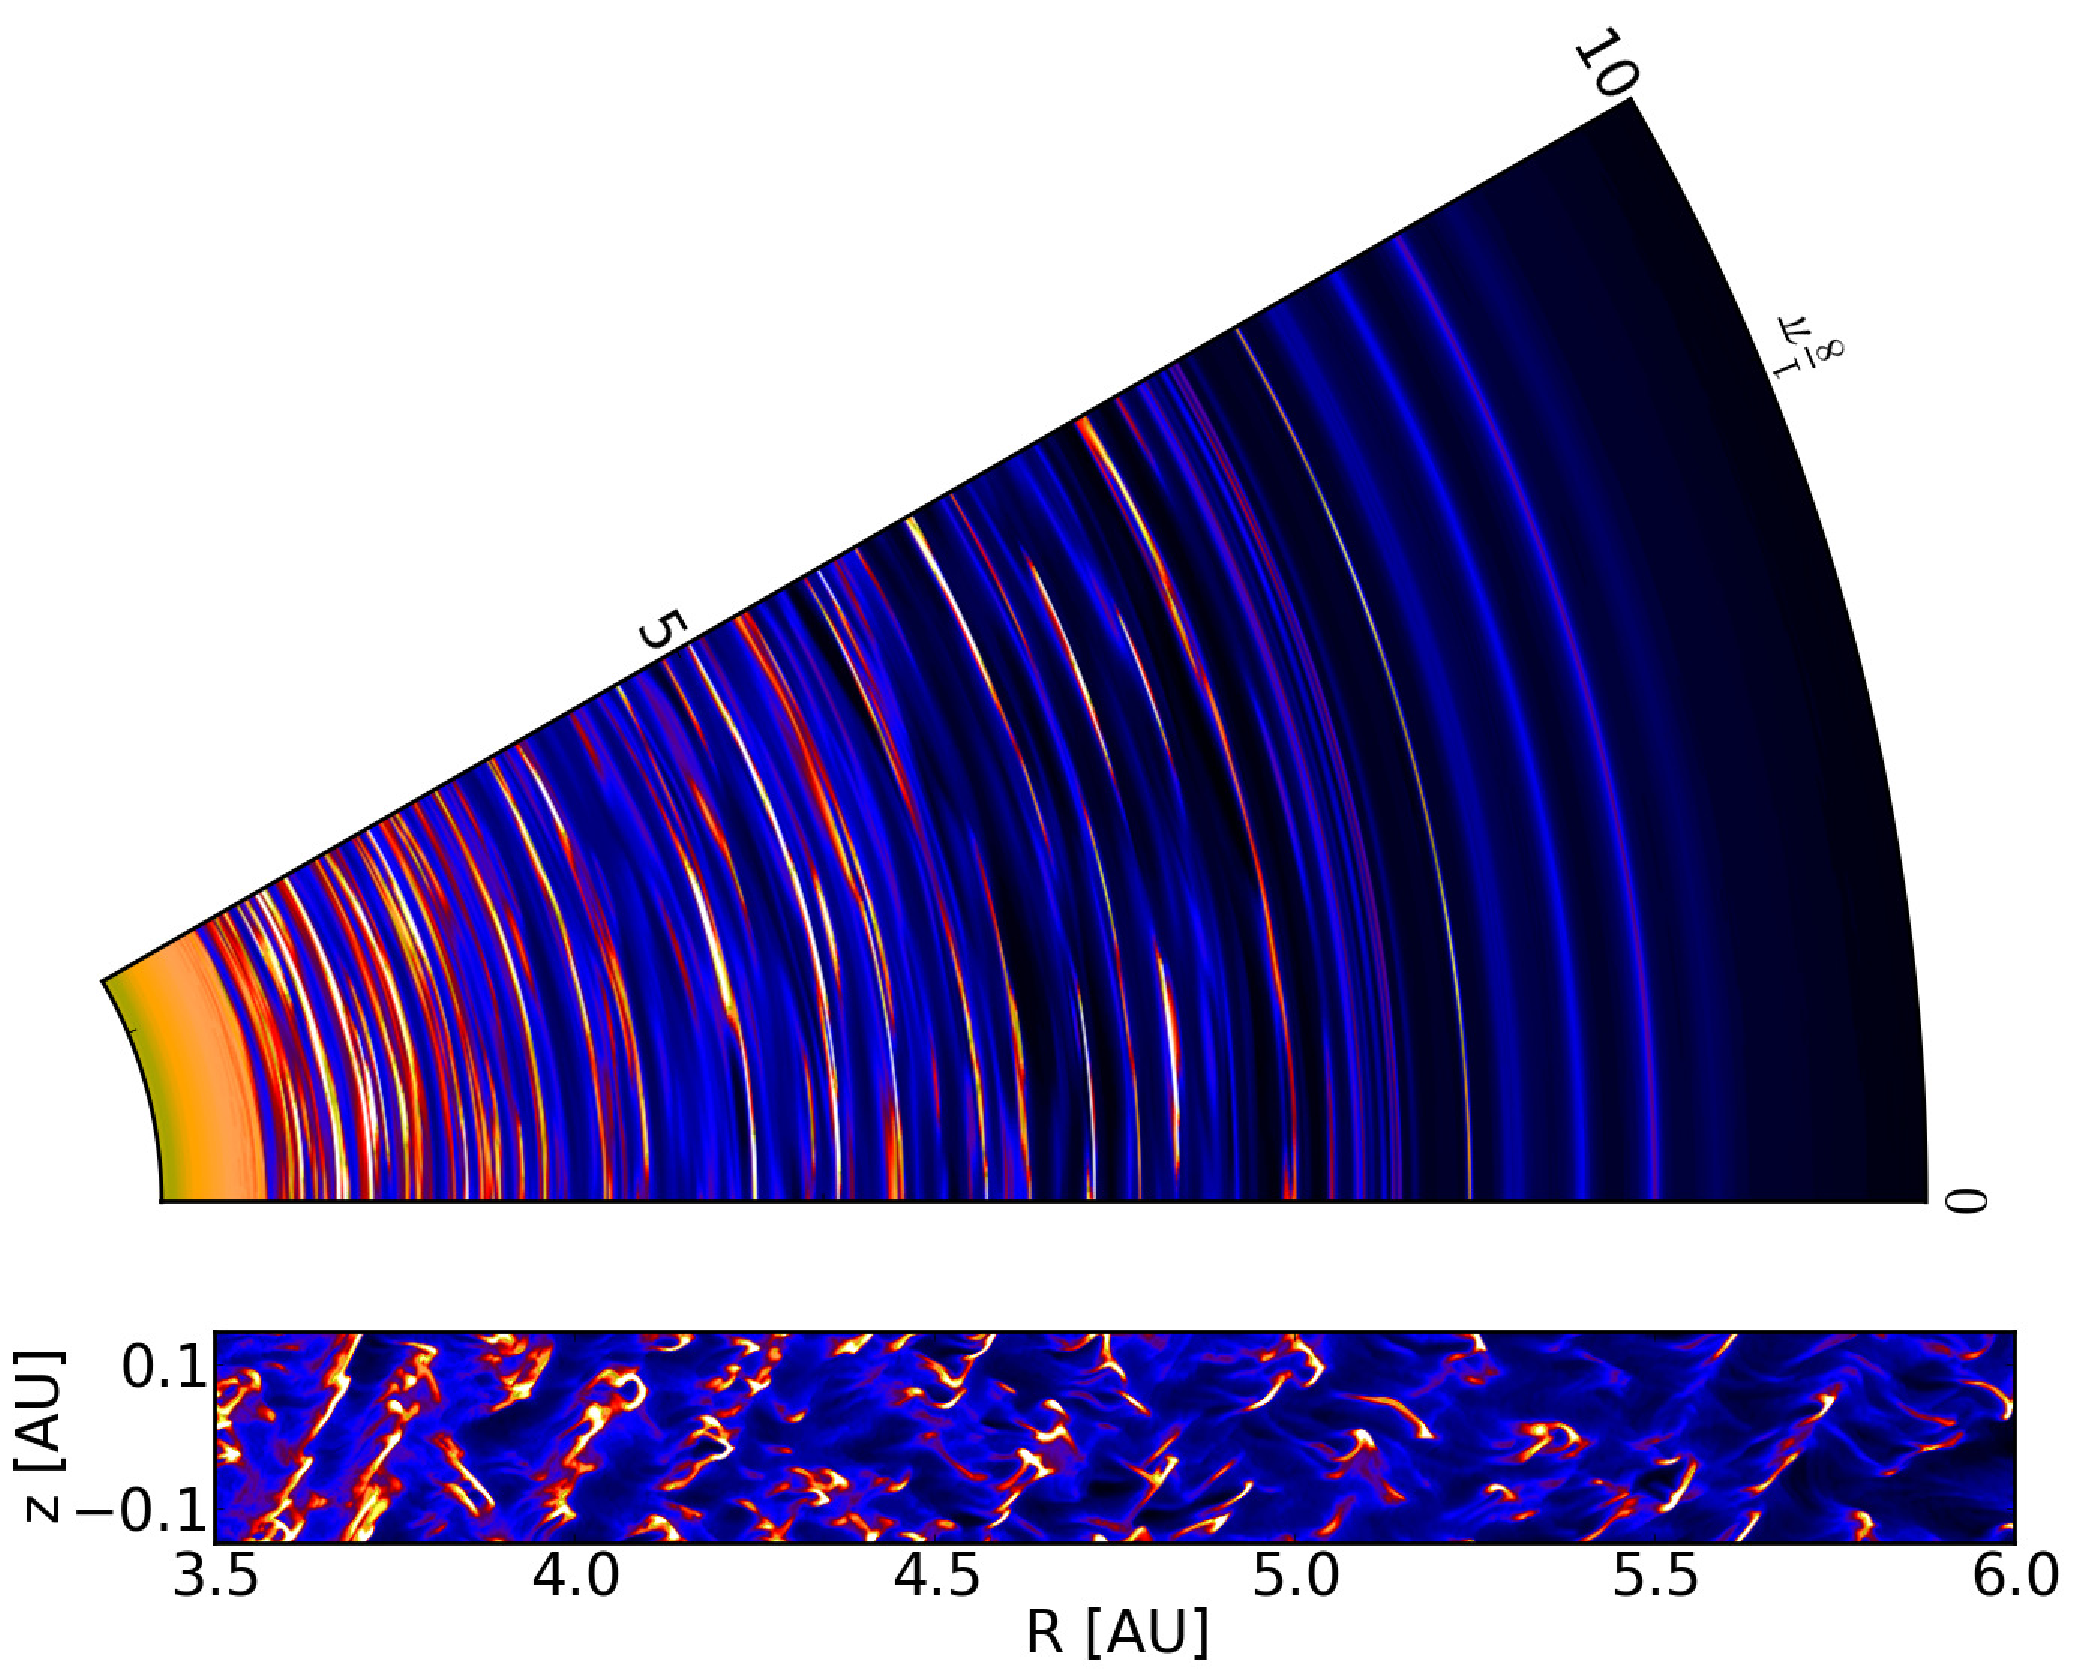
\includegraphics[width=0.98\linewidth]{figures/fig5}
   \caption{Snapshot of dust density distribution from run BB3D taken at
   $t=500$~yr. Upper panel shows a slice through the disc midplane, whereas lower
   panel is a part of slice perpendicular to disc plane zoom out to the region
   that corresponds to physical span of 2D simulations.}
   \label{fig5}
\end{figure}
In order to estimate whether we should expect effects of self-gravity  in the
nonlinear evolution of streaming instability, we have used \yt{}~\citep{yt} clump
finding facility to identify all the largest disconnected contour spanning for
minimum value of 50 computational cells in BB3D run. Then we calculated their
total mass and velocity dispersion $\sigma$ to obtain Jeans' radius:
%
\begin{equation}
   R_J = 2 GM / \sigma^2.
\end{equation}
Subsequently we compared the average size of each individual clump $L =
\sqrt{\sum_{i\in{\{x,y,z\}}} \max (L_i^2)}$ and found that $L < R_J$ for every
identified overdense clump, indicating that the clumps fulfill the gravitational
binding condition (see Fig.~\ref{fig6}). This indicates that in certain
situations, i.e. for dust dominated runs of the semi-global disc configuration,
streaming instability acting in a selfgravitating medium can lead to planetesimals
formation~\citep{J07}.

\begin{figure} 
  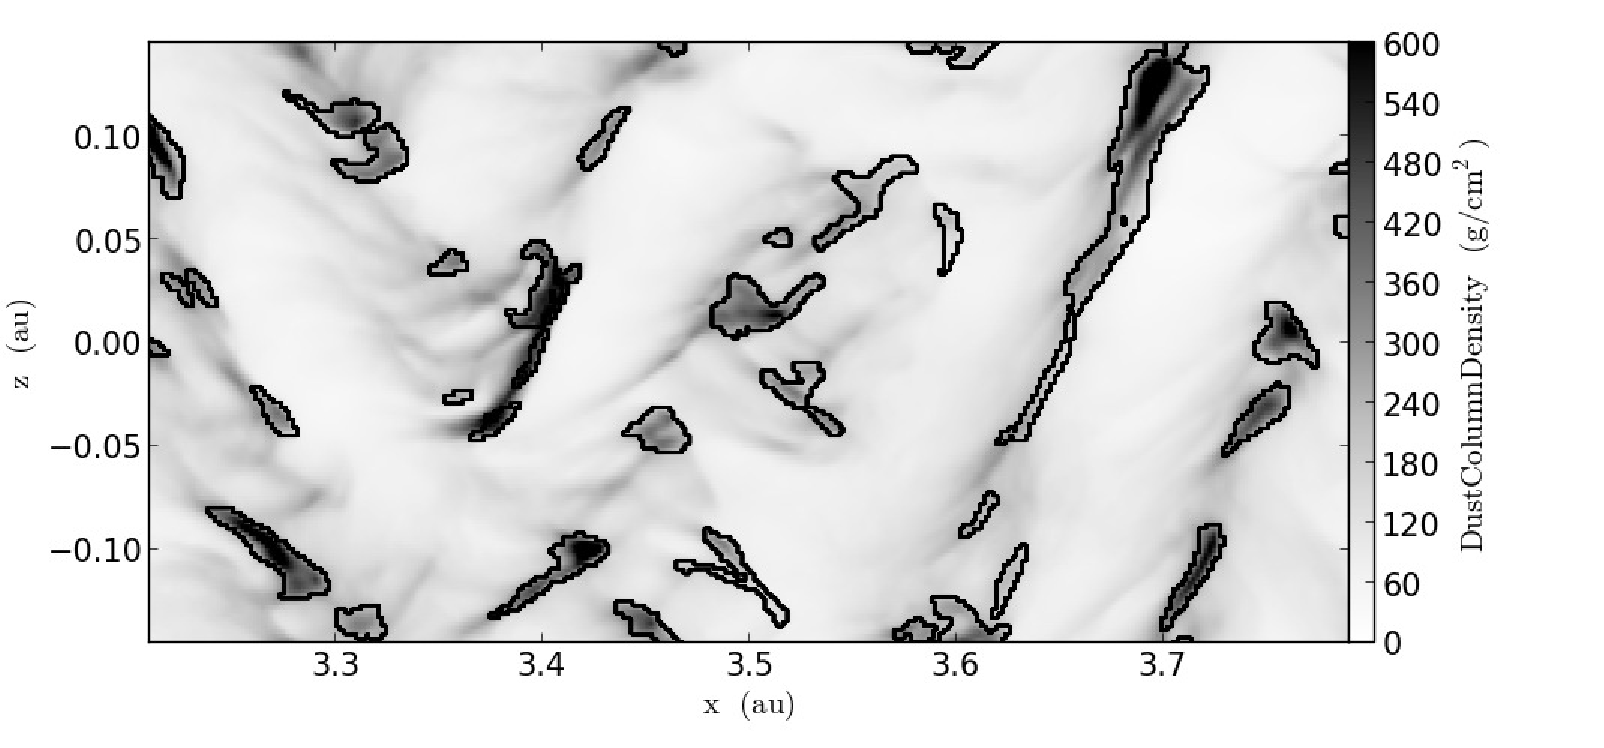
\includegraphics[width=0.98\linewidth]{figures/fig6}
  \caption{
     Small patch showing projection of dust density along azimuthal axis from
     run BB3D with annotated contours of gravitationally bound clumps.}
  \label{fig6} 
\end{figure}

\subsection{Comparison to the Results of Linear Stability Analysis}
In order to analyse the growth of streaming instability we extract small square
patches from various locations across the computational domain. The patches have
sizes of $0.15^2$~AU$^2$, thus are small enough so that mean values of physical
quantities do not vary significantly across them. In the case of 3D run the
patches are chosen on the {\it r-z} plane at $\varphi = \varphi_\textrm{max} /
2$. 

We note that in the place of the fixed parameters  describing the unperturbed
equilibrium  in \mref{lin1}--\mref{lin2}, we use patch-averaged values of
corresponding dependent variables in equations \mref{eqc1}--\mref{eqm2}. 
We calculate the spatially averaged densities of gas and dust component
$\bar{\rho}_g = \left<\rho_g\right>$, $\bar{\rho}_d = \left<\rho_d\right>$ and
their mutual ratio $\bar{\epsilon} = \left<\rho_d / \rho_g\right>$ . Mean
angular velocity $\bar{\Omega}$ is taken for the center of the patch.
Dimensionless measure of sub-Keplerian gas rotation is calculated by means of
the formula~(see YG05 eq.~(16) or JY07 eq.~(1))
%
\begin{equation}
   \bar{\eta} = -\frac{c_s^2\left<\partial_R \left<\rho_g\right>_z\right>_R}
      {2\bar{\rho}_g\bar{\Omega}^2 R},
   \label{eq:eta}
\end{equation}
%
In formula \mref{eq:eta} we average gas density in the vertical direction, then
we calculate the mean radial derivative of $\left<\partial_R \rho_g\right>$. 
The expression for mean stopping time is derived from \mref{eq:tauf}
\begin{equation}
   \bar{\tau}_f = \rho_\bullet a / \left(\bar{\rho}_g \sqrt{c_s^2 +
   \left<\left|\mathbf{u} - \mathbf{v}\right|^2\right>} \right).
\end{equation}
%
For the sake of consistency gas and dust velocities $\bar{\mathbf{u}},
\bar{\mathbf{w}}$ are also approximated by their mean values
$\left<\mathbf{u}\right>, \left<\mathbf{w}\right>$ instead of calculating them
with the aid of \mref{eq:w0}-\mref{eq:u0}. However, we note that the mean values
that are naturally achieved during the simulation,  do not diverge from the
equilibrium solution by more than $10\%$. 

To determine linear growth rates of the excited instability modes we calculate
Fourier transforms of density and velocity distributions of the dust component.
We analyse subsequently time variation of amplitudes of individual modes.
Intermediate results are shown in Fig.~\ref{fig7}. 

\begin{figure}
  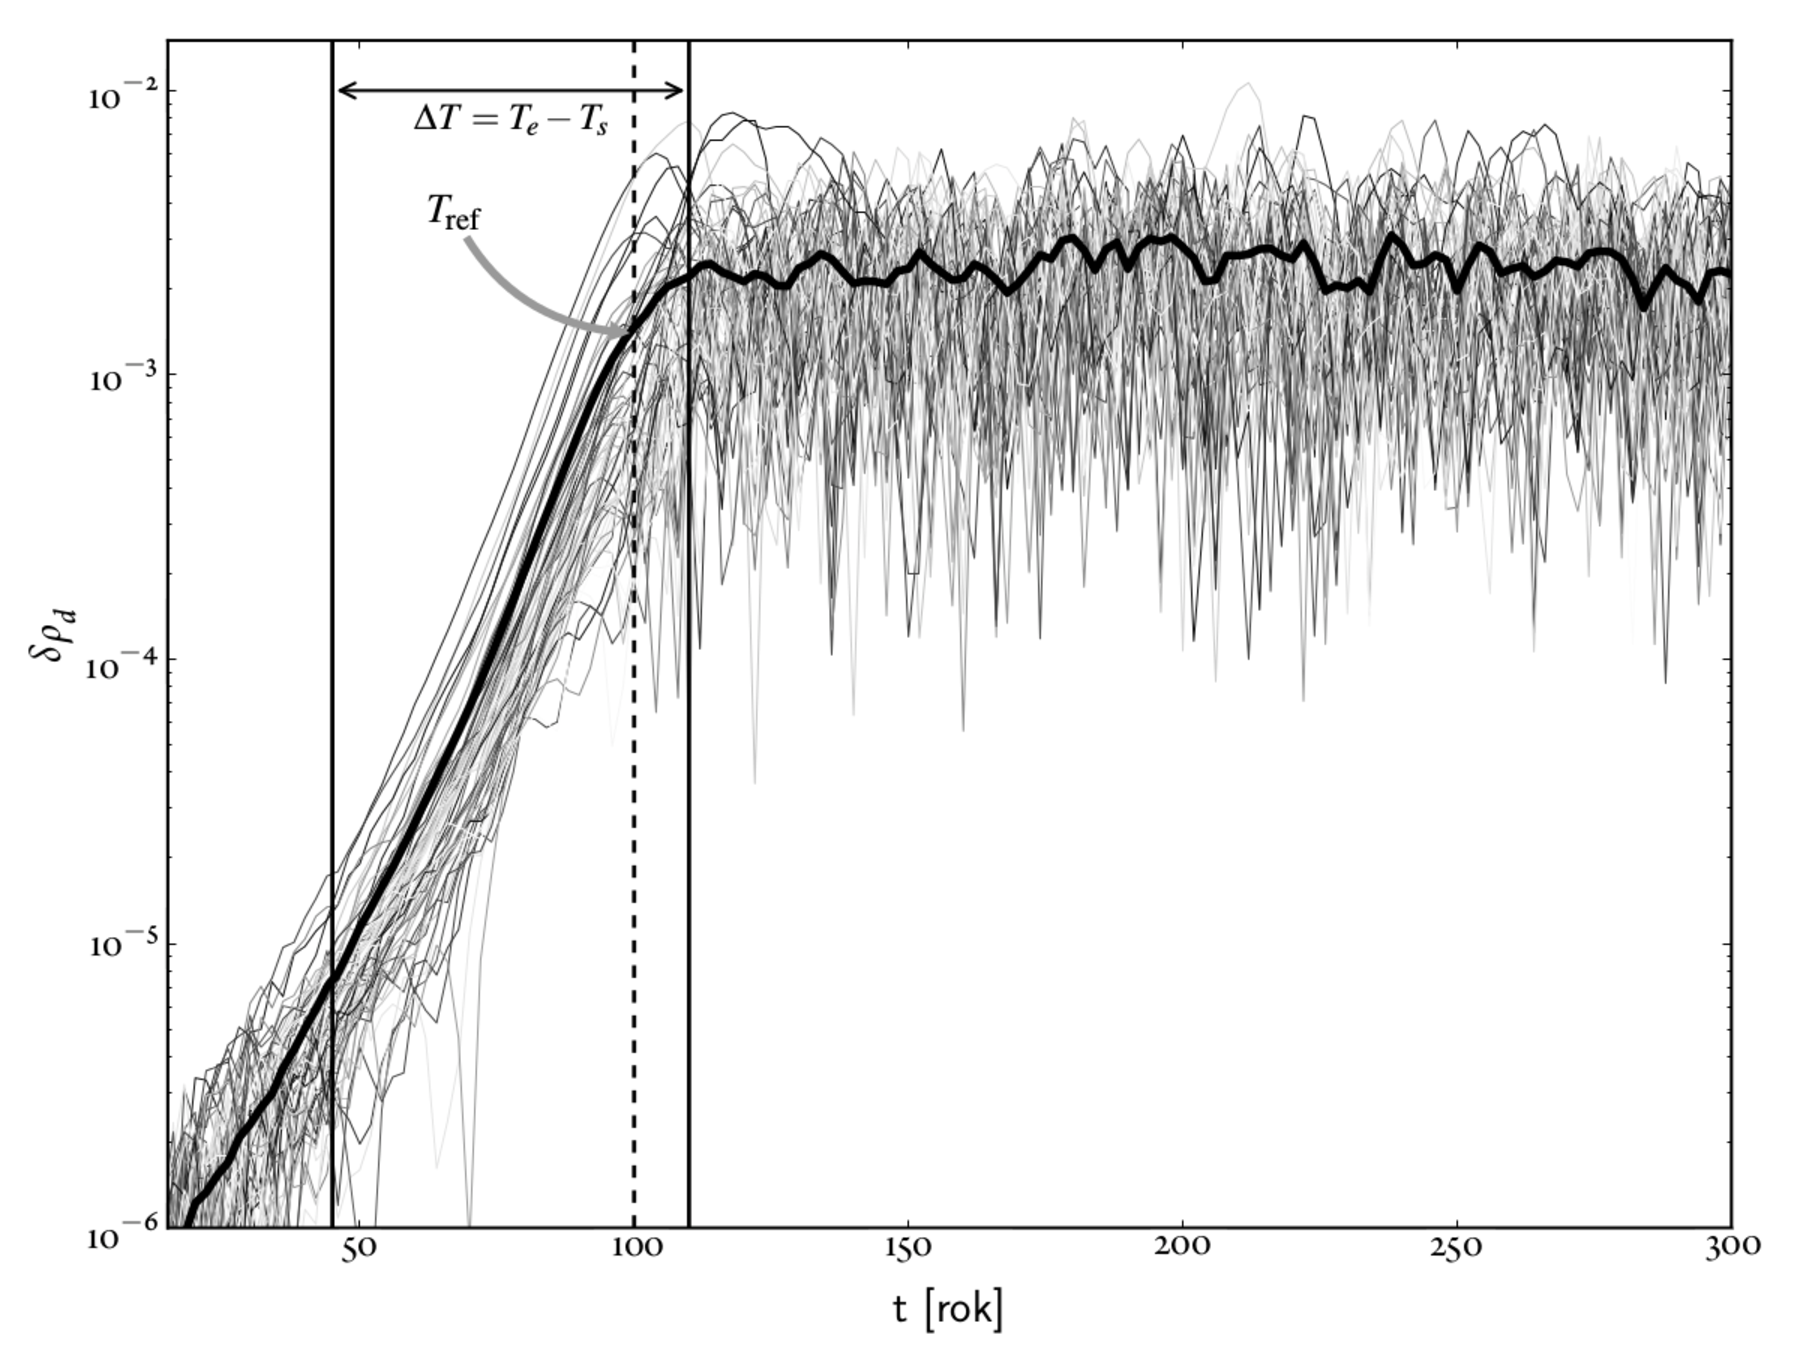
\includegraphics[width=0.98\linewidth]{figures/fig7}

  \caption{Temporal evolution of dust density perturbation amplitude in the
     Fourier space in the patch located at $[2.85,3.15]\times[-0.15,0.15]$~AU
     from simulation BB.  Each line represents amplitude for a given pair of
     $k_x, k_z$.  $\Delta T = T_e - T_s$ is time range when modes are fitted
     with \mref{eq:fit}.  $T_{\textrm{ref}}$ is a reference point in time used
     to identify most dominant modes using criterion of maximum amplitude value.
     Thick line is an average of amplitudes that are grater than $10^{-4}$ at
     reference time $t = T_{\textrm{ref}}$
   } 
   \label{fig7} 
\end{figure}

We identify time $T_s$ at which the dominating modes emerge from fluctuations
and start their linear growth phase. Similarly, we identify the end of the
linear growth phase $T_e$ when modes have grown by few orders of magnitude, and
start to saturate their growth. We fit exponential function:
%
\begin{equation}
   f(t) = A\exp\left(-s t\right)
   \label{eq:fit}
\end{equation}
%
 to the measured density amplitudes in the  period $\Delta T = T_e - T_s$.

That procedure allows us to determine the growth rate $s(k_x, k_z)$ of each
individual unstable mode, during the linear phase of the instability growth in
the numerical experiments.  We identify the most rapidly growing modes by
selecting those with the greatest amplitude at fixed point at the reference time
$T_{\textrm{ref}}$ before the saturation. We compare the growth rates $s(k_x,
k_z)$ obtained for each mode  with the solution $s_0(k_x, k_z)$ resulting from
the linear analysis for the local mean flow parameters. 

In Fig.~\ref{fig8} we show temporal evolution of dust density perturbation
amplitudes for three dominating instability modes in three experiments BB3d, BB
and BBh, together with lines fitted to the phase of linear growth and  lines
representing growth of the amplitudes predicted by the linear analysis of the
streaming instability.  In the mid resolution run BB the growth rates  are
$10\div30\%$ smaller than those predicted by linear analysis, what indicates
that still higher resolution is required to resolve these modes. In the high
resolution run BBh the results of the numerical experiment tend to converge the
results of linear stability analysis.  The final saturation amplitudes seem to
be slightly smaller in high resolution runs. One should note, however, that we
have chosen the modes of the highest growth rate for each run, which are not the
same modes in terms of wavenumbers. 
 
\begin{figure} 
   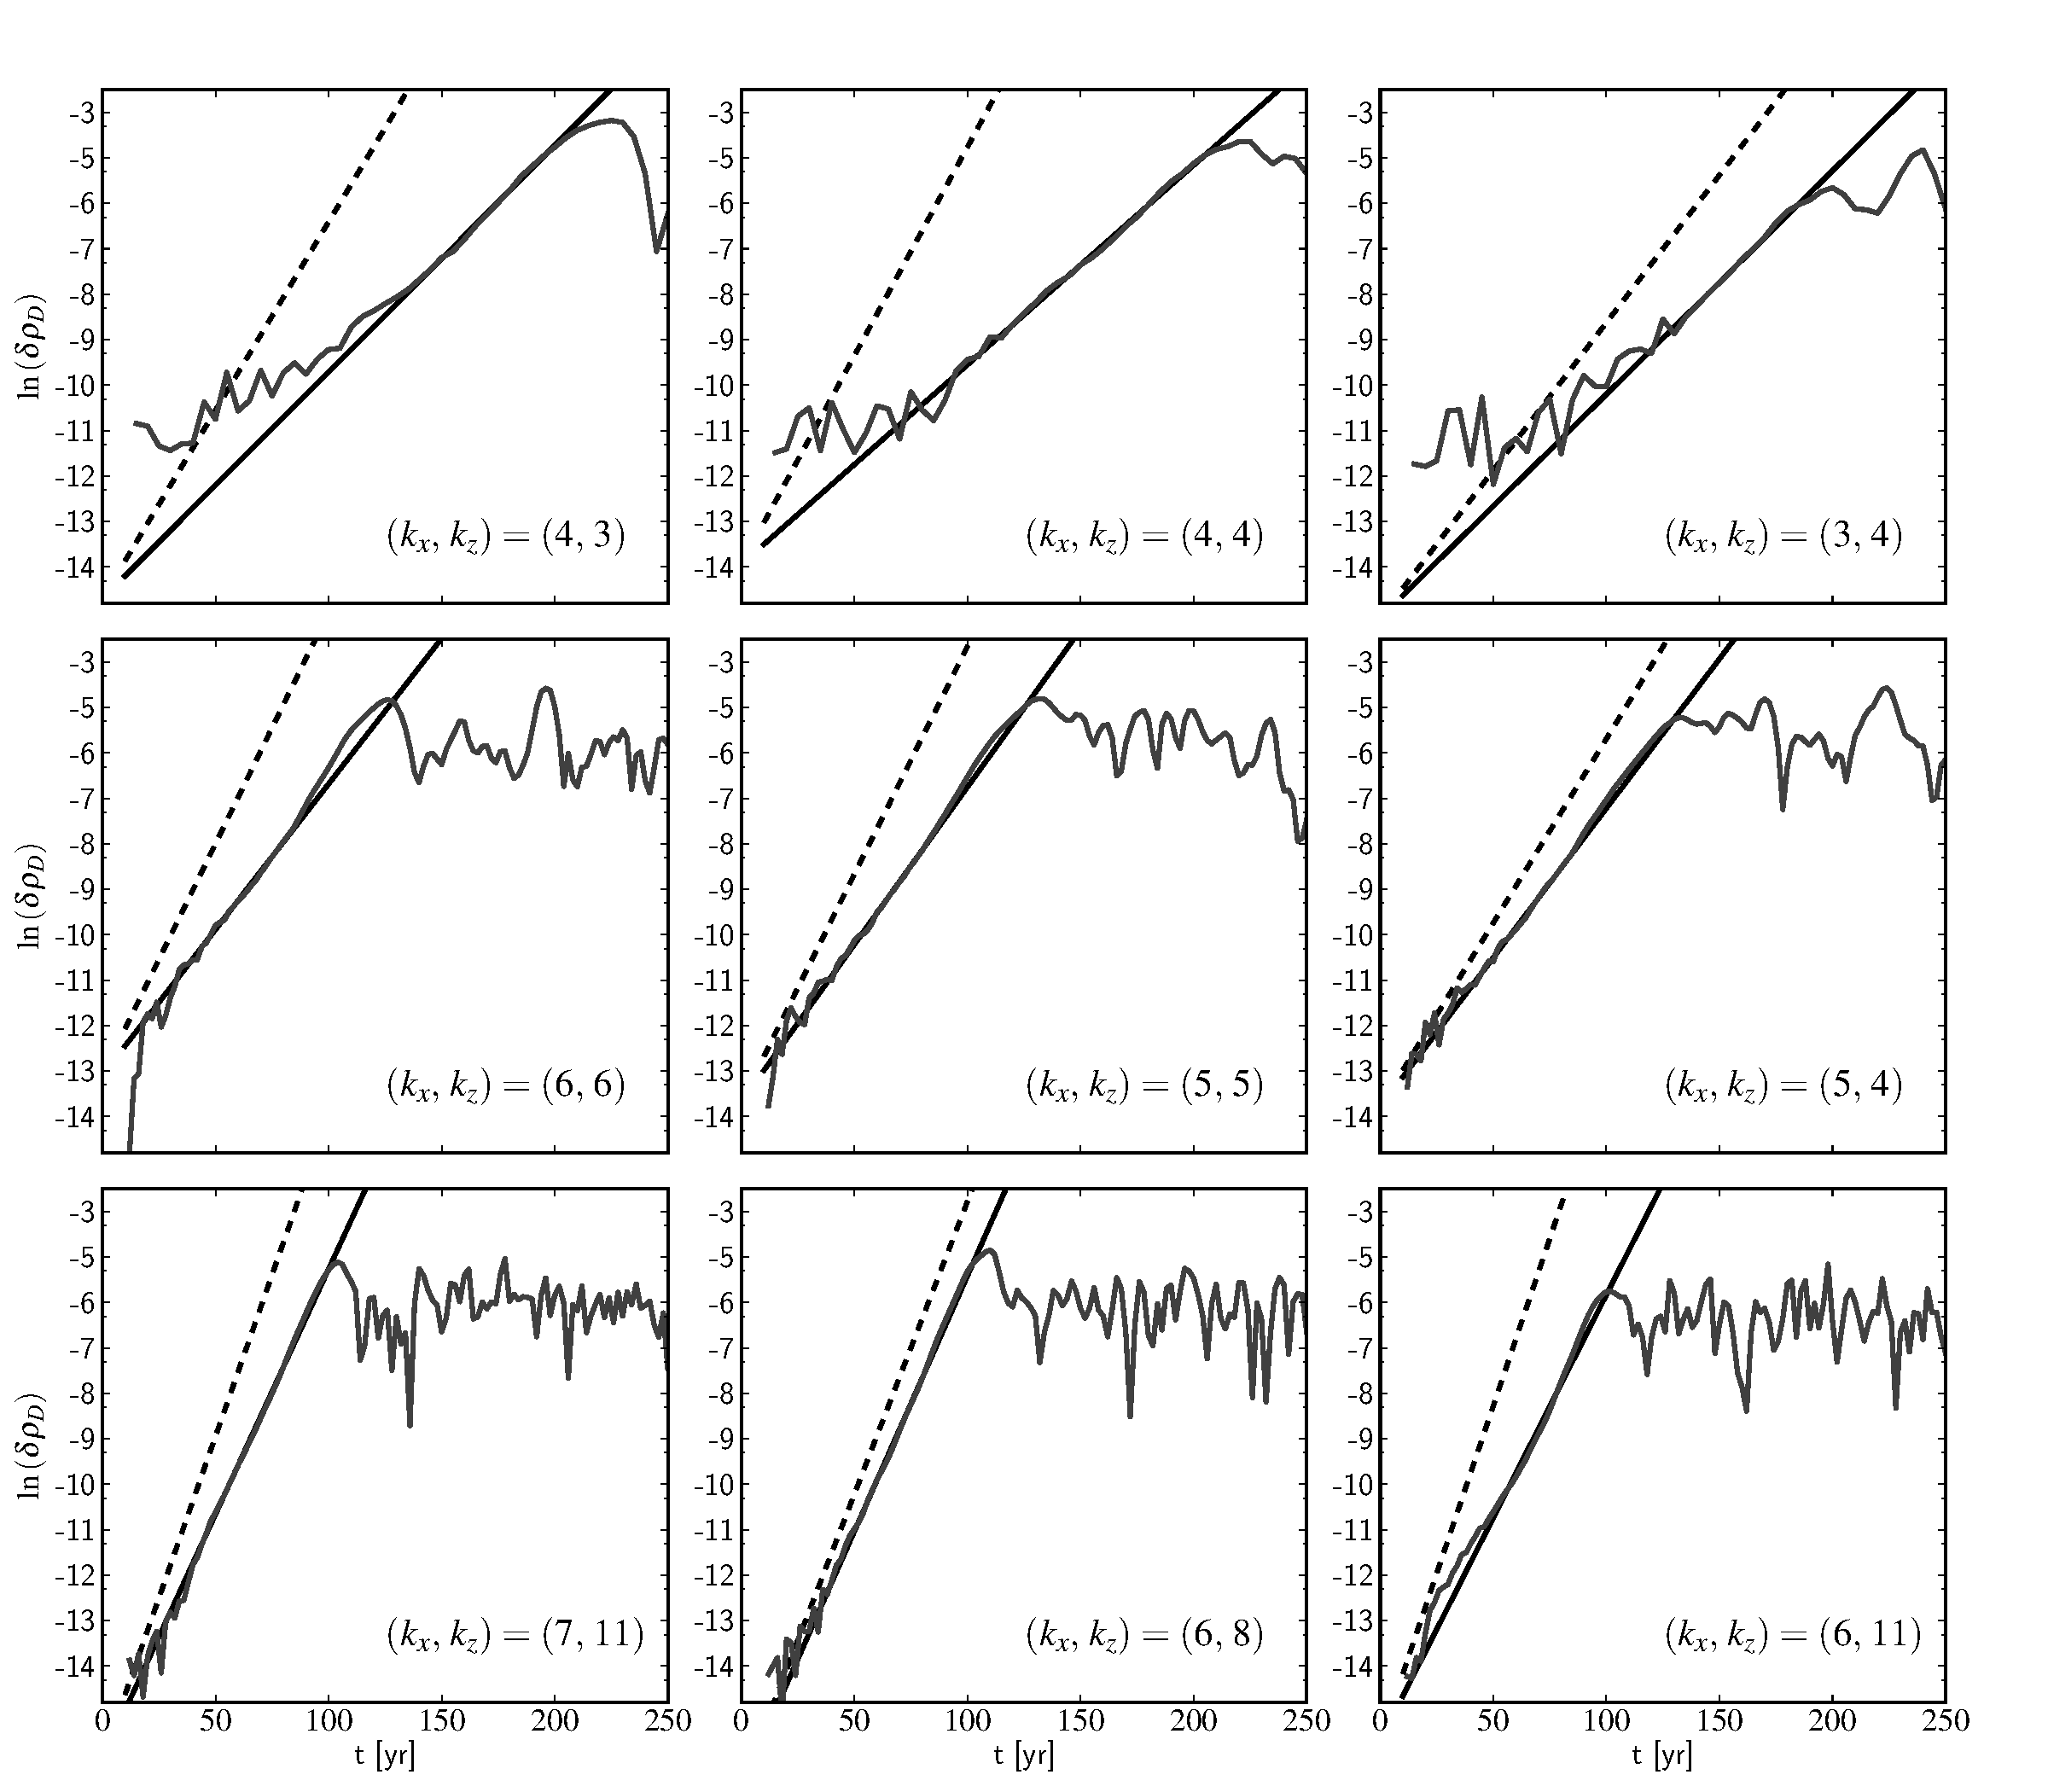
\includegraphics[width=0.98\linewidth]{figures/fig8}
   \caption{Temporal evolution of the amplitudes of the dominating instability
      modes, measured in the dust density (gray line) together with the lines
      resulting from the linear analysis of the streaming instability (dashed
      line) and lines of fits of eq.~\mref{eq:fit} to the measured amplitudes
      (black lines).
      The linear solution of eq.~\mref{eq:linset} is found for the mean
      parameters of the rectangular patch at $R=3$~AU for the simulations: BB3d
      (upper panel), BB (middle panel) and BBh (lower panel). 
   }
   \label{fig8}
\end{figure}

\par To extend our analysis we show in Fig.~\ref{fig9} a contour plot
(following YG05 and YJ07) of the growth rate  $s(k_x, k_z)$, resulting from
solutions of the dispersion relation \mref{eq:disprel}.  The shape of
isocontours indicates that the most unstable modes of the streaming instability,
predicted by linear analysis, form a ridge extending towards  large values of
$k_x$ and $k_z$.  The plots are constructed for the same set of the physical
parameters and the mean state parameters derived for  the domain patches at $T=T
_{\textrm{ref}}$.  We then place  $(k_x, k_z)$ of 9 dominating modes extracted
at $T = T_{\textrm{ref}}$  for simulations performed at different resolutions.

Our procedure allows us to confirm that  wavenumbers  of the modes, emerging in
presented numerical models, align with the  ridge of linear solutions at the
growth rate map.  It is apparent that dominating modes  are limited by available
numerical resolution. At lower numerical resolutions (run BB3d)  the dominant
modes locate below the contour labeled as ''$-1.000$''. At the mid resolution of
run BB some of the modes locate above the contour ''$-1.000$'', and at the high
resolution most of the modes locate above this contour. Similar tendency can be
observed for the pair of runs AB and ABh.  We anticipate that the reason for the
absence of the very short wavenumber modes is the numerical diffusivity of the
presently  used Relaxing TVD algorithm. Our estimations show that  our code
requires at least 32 computational cells per wavelength of the unstable mode, to
accurately represent the linear growth rate, which is much more than is required
by higher-order schemes~\cite{YJ07, BT09}.


\begin{figure*}
  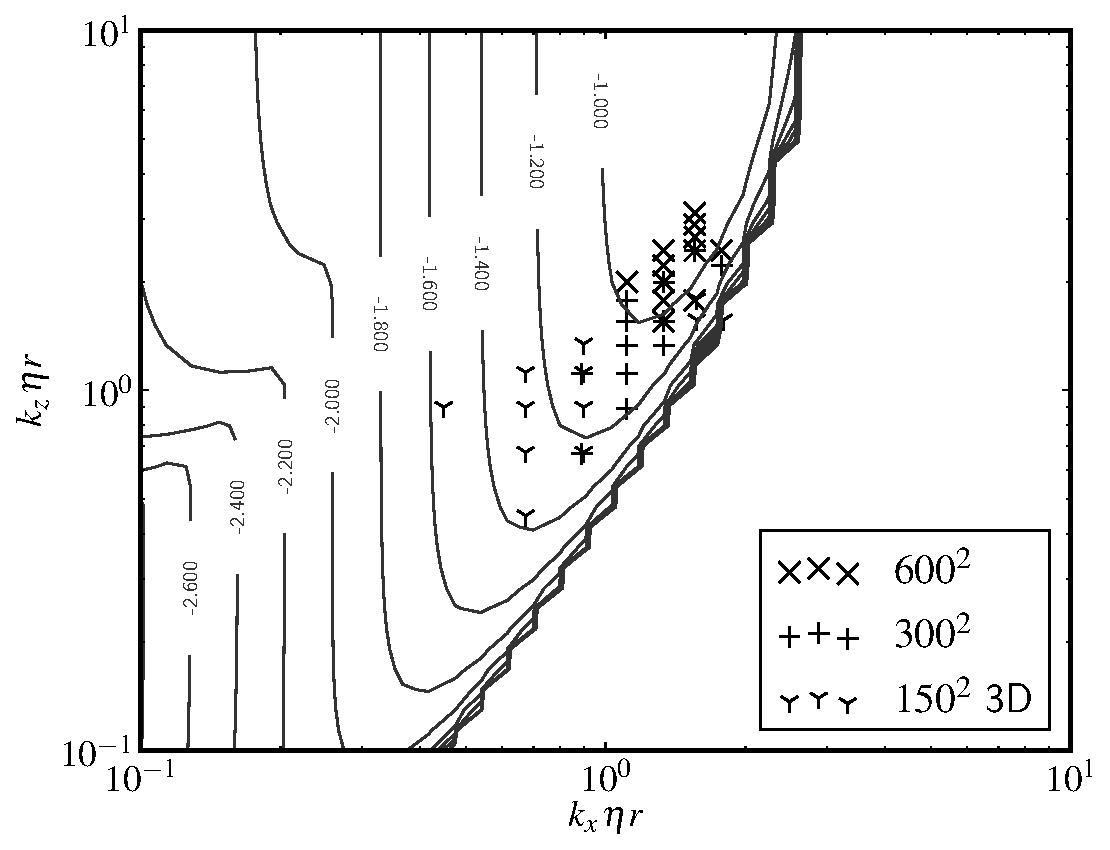
\includegraphics[width=0.48\linewidth]{figures/fig9a}
  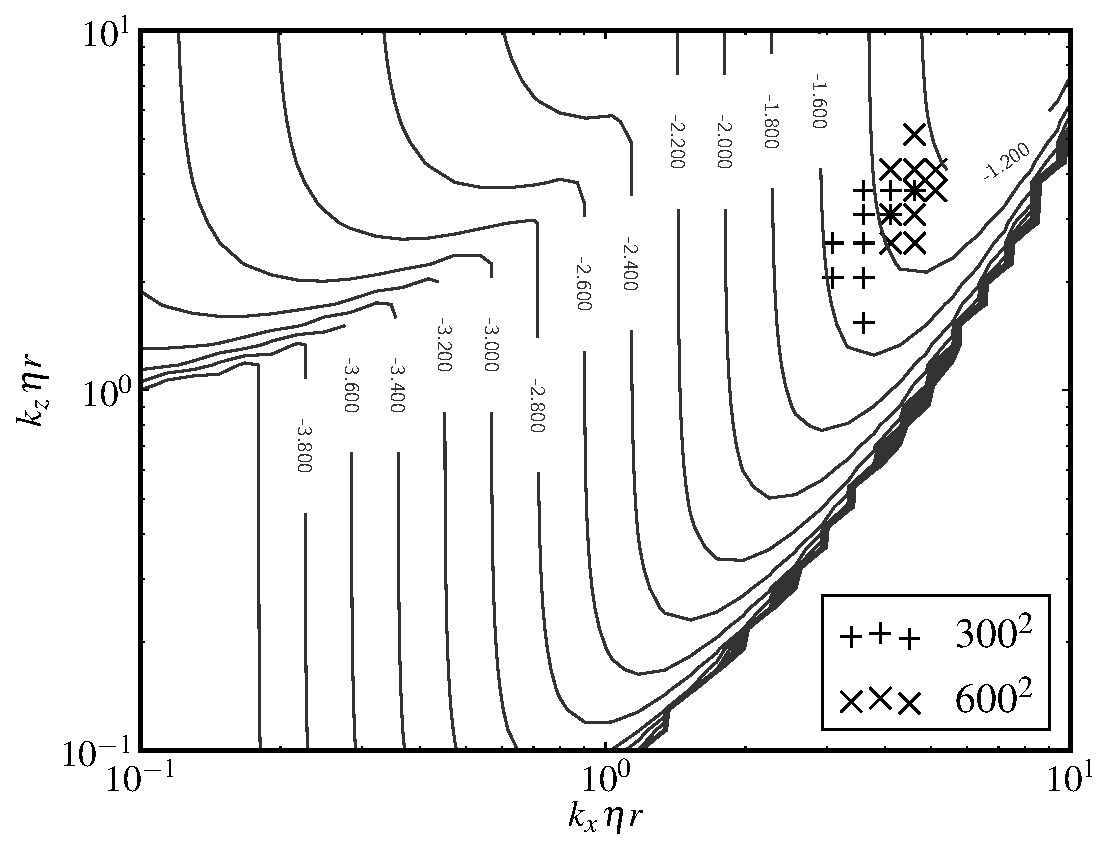
\includegraphics[width=0.48\linewidth]{figures/fig9b}
  \caption{
     The nine of the fastest growing modes characterized by wavenumbers
     $(k_x, k_z)$ extracted  from different simulations sharing the
     same initial conditions (left panel: BB, BBh, BB3d, right panel: AB, ABh)
     but different resolutions. Contours of growth rates $\log_{10}( s(k_x,
     k_z))$  represent solutions of \mref{eq:disprel} for the mean state
     parameters derived for  the domain patches at $T = T_{\textrm{ref}}$
  (for comparison see Fig.~2 of YG05)}
   \label{fig9}
\end{figure*}
 
% \subsection{Convergence}
We varied the resolution of our simulations to check how our numerical scheme
affects the obtained solutions. As the streaming instability in general
"prefers" shorter wavelengths for the optimal growth, increasing resolution
always leads to more, smaller overdensities emerging during the course of
evolution (see Fig.~\ref{fig10}). However we note that our results
follow the fastest growing, linear modes (see Fig.~\ref{fig9}) and
that most phenomena described in previous sections i.e. cavitation (see
Fig.~\ref{fig3}) or sudden growth dumping of the tightly coupled
boulders in the gas dominated regime (see Fig.~\ref{fig4}) are independent of
the size of the smallest computational cell.

\begin{figure}
   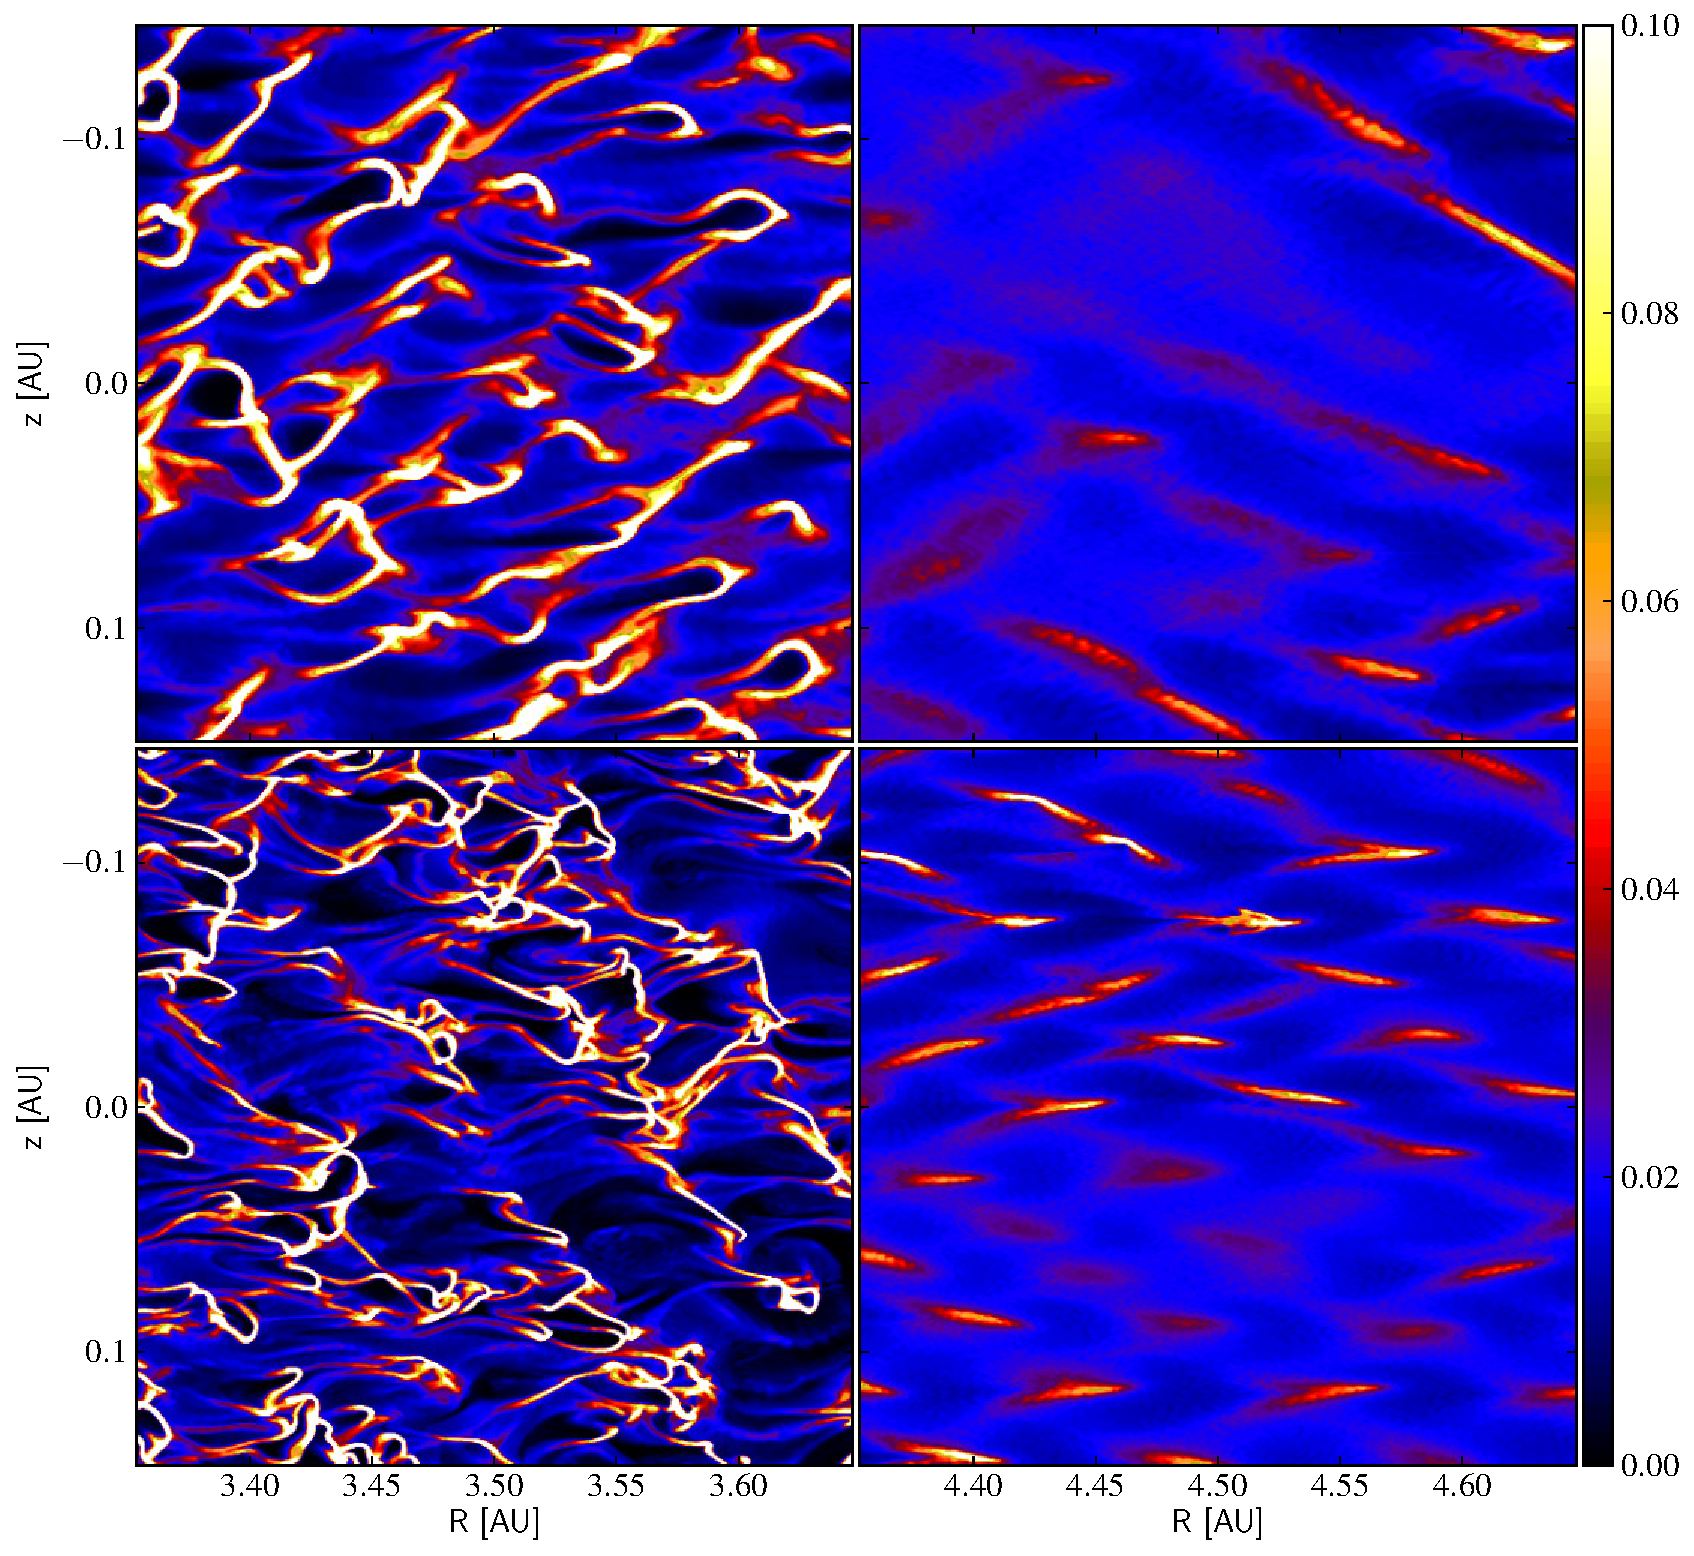
\includegraphics[width=0.98\linewidth]{figures/fig10}
   \caption{Dust density snapshots at $t = 160$~yr in two small rectangular
      patches for the two identical simulations parameters (upper: BB, lower:
      BBh) showing how the resolution affects simulation results at the linear
      and saturation phase of the instability. It is apparent that shorter
      wavelength modes dominate at the higher resolution, and that dust
      condensation structures are sharper.
   } 
   \label{fig10} 
\end{figure}
